\documentclass[a4paper,11pt]{style-esi/td}

\usepackage{style-esi/licence}	% Affiche une licence dans le document
\usepackage{style-esi/exercice}
\usepackage{style-esi/listing}
\usepackage{style-esi/tutoriel}
\usepackage{style-dev1/dev1}
\usepackage{terminal}
\usepackage[french]{varioref}
\usepackage{newunicodechar}
\usepackage{xspace}
\newunicodechar{ }{~}
\newunicodechar{ }{\,}
\newunicodechar{…}{\ldots}

\marginnumbertrue

\newcommand{\git}{\textbf{git}\xspace}

\begin{document}

\seance{5}{Git - Console}
\entete
\titre
\ccbysa{esi-dev1-list@he2b.be}
\lastedit

\bigskip

Un logiciel de gestion de versions est un outil permettant de conserver
l’historique des modifications apportées à un projet (code source,
documentation, etc.).

L’entièreté de l’historique étant conservé, les fichiers peuvent être comparés
avec n’importe quelle version précédente.  Un tel logiciel permet également de
maintenir les modifications d’un code source cohérentes à travers le temps, en
particulier si on travaille en équipe. Lorsque deux développeurs modifient un
même fichier, ils en seront notifié pour éviter que l’un écrase le travail de
l’autre. Ils pourront alors fusionner leurs codes ensemble.  L’utilisation d’un
logiciel de gestion de versions est devenue essentielle dans une équipe et est
très appréciable lorsque l’on travaille seul. 

Il existe une multitude de logiciels de gestion de versions, dont l’un s’est
démarqué au cours de la dernière décennie : \textbf{git}.  


\begin{alertit}{Préalable}
	Nous supposons dans ce TD que le TD «~Git - Netbeans~» a été réalisé. 
\end{alertit}

\tableofcontents
\newpage


\section{Vocabulaire}

Pour permettre l’accès à l’historique d’un projet, \git doit conserver toutes
ces données de manière structurée. L’espace de stockage contenant toutes ces
données est nommé \textbf{dépôt} (\textit{repository}). 

Les éléments principaux composant un dépôt sont les \textbf{soumissions}
(\textit{commits}).  Chaque \textit{commit} contient l’ensemble des fichiers et
leurs contenus qui composaient le projet à un moment donné. Un commit contient
également une série de méta-données comme une date de création, le nom du
créateur et une description. Pour pouvoir les identifier, les \textit{commits}
possèdent tous une clé unique. 

Pour partager facilement un dépôt entre plusieurs personnes, celui-ci doit leur 
être accessible. Pour faciliter cette gestion et l'hébergement d’un dépôt, 
plusieurs services web ont vu le jour pour conserver un dépôt centralisé. 
Citons \textit{Github}, \textit{GitLab}, et \textit{Bitbucket}. 


\subsection{Exemple}

\begin{figure}[h]
	\centering
	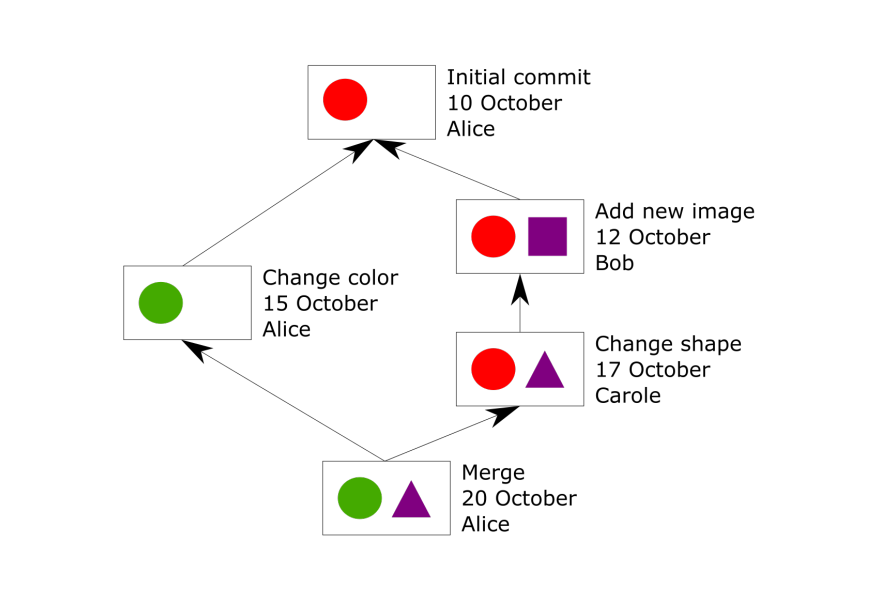
\includegraphics[width=.9\linewidth]{img/exemple.png}
	\caption{Exemple d'évolution d'un projet.}
	\label{fig:exemple}
\end{figure}

La figure \vref{fig:exemple} illustre l’évolution possible d’un projet. 

\begin{enumerate}

	\item Alice crée d’abord un premier \textit{commit} avec un fichier simple~: 
		l’image d’un cercle rouge. 
		
	\item Ensuite, Bob ajoute un nouveau \textit{commit} avec l’image d’Alice et un 
		nouveau fichier contenant un carré mauve. 
		
	\item Carole modifie le carré mauve de Bob en triangle. 
		
	\item Pendant ce temps, Alice, dans un nouveau commit, change la couleur de 
		son cercle, sans être au courant des changements de Bob et Carole. 
		
	\item Enfin, les deux équipes se rendent compte de leur dispersion et créent 
		un nouveau \textit{commit} avec les améliorations de chacun. 

\end{enumerate}

\begin{theorie}{Commande git}
	Une commande \git est de la forme~:

	\bigskip
	\texttt{\Large git <command> [options]}
	\bigskip

	À chaque commande (\texttt{command}) correspond des options éventuelles
	(\texttt{options}).

\end{theorie}


\section{Mise en place}

Lorsque plusieurs personnes travaillent ensemble, elles peuvent centraliser
leurs dépôts sur internet. Par exemple sur un serveur \textit{Gitlab}. 

Ces personnes peuvent donner la possibilité à d'autres de copier tout leur
dépôt. Cette copie sera un dépôt complètement indépendant du premier. On parle
de \textit{fork}.  

\bigskip
\begin{colxbox}[colback=white,drop fuzzy shadow]

	Nous travaillons avec le dépôt
	\url{https://git.esi-bru.be/dev1/labo-envl-git} 
	qui est en lecture seule et
	que nous vous invitons à \textit{forker}.

\end{colxbox}
\bigskip

\begin{figure}[h]
	\centering
	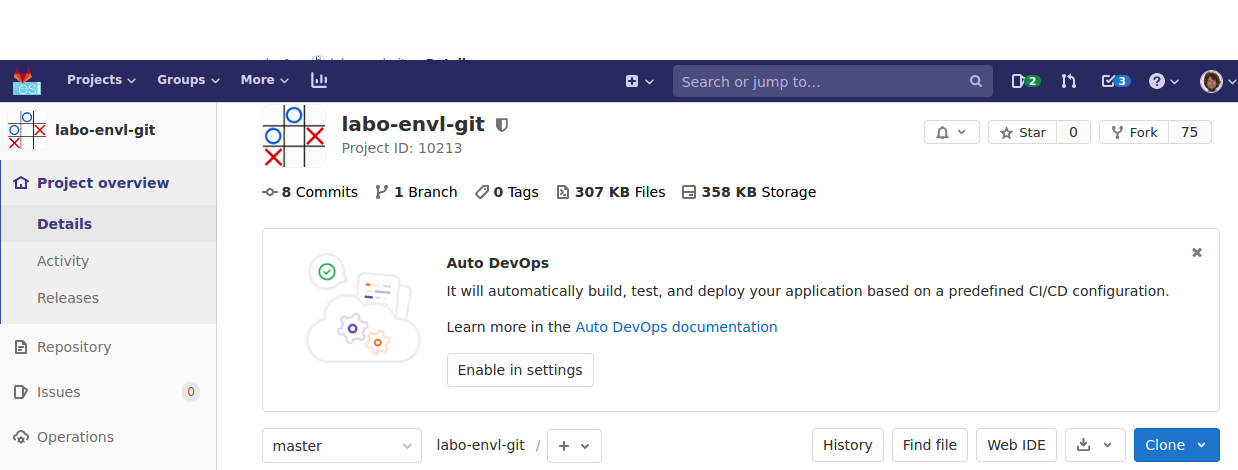
\includegraphics[width=.9\linewidth]{img/depot-git-1.png}
	\caption{Dépôt git à l'adresse \url{https://git.esi-bru.be/dev1/labo-envl-git}}
	\label{fig:depot}
\end{figure}

\begin{Exercice}*{Forker le dépôt}
	\begin{steps}

	\item Se rendre à l'adresse 
	\url{https://git.esi-bru.be/dev1/labo-envl-git}. Forkez le projet en cliquant
	sur le bouton idoine.
	\begin{center}
	
\includegraphics[scale=0.6]{img/depot-git-2.png}
	\end{center}
	
	\item Prenez note de l'adresse du \textit{fork} qui sera de la forme~:\\
	\url{https://git.esi-bru.be/<votre login>/labo-envl-git}.

	À cette adresse, vous trouverez l'adresse de votre dépôt dans deux
	protocoles différents~: \texttt{ssh} et \texttt{https}. Voir les images à la 
	figure \vref{fig:depot-git-3}.

	\begin{figure}[h]
		\centering
		
\includegraphics[scale=0.6]{img/depot-git-fork-1.png}
		\caption{Un dépôt git a deux liens : https et ssh}
		\label{fig:depot-git-3}
	\end{figure}

	\end{steps}
\end{Exercice}

Pour travailler localement sur un dépôt, il est nécessaire de le \textbf{cloner}
c'est-à-dire rapatrier son contenu sur la machine pour y avoir accès. 
C'est la commande \texttt{clone} de git qui s'en charge. 

Cette commande crée un répertoire et copie le dépôt. Dans le répertoire copié
se trouve un sous-répertoire \texttt{.git} contenant tout ce qui concerne git. 

\begin{Exercice}*{Cloner le projet localement}
	\begin{steps}
		
	\item Clonez le dépôt \texttt{labo-envl-git} dans le répertoire courant en
		utilisant l'adresse de votre fork commençant par \texttt{https}. 

		\begin{term}
			git clone https://git.esi-bru.be/login\footnote{Remplacer 'login' par votre login}/labo-envl-git
		\end{term}

		Git vous demande vos identifiants. Entrez les.  

	\item Constatez la présence d'un nouveau répertoire \texttt{labo-envl-git} dont le contenu à l'allure de la figure \vref{fig:tree}

		\begin{figure}[h]
			\centering
			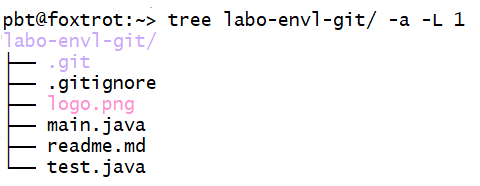
\includegraphics[width=.7\linewidth]{img/tree.png}
			\caption{Contenu du répertoire après clone}
			\label{fig:tree}
		\end{figure}
	
	\end{steps}
\end{Exercice}

Par défaut \git utilise vos nom et email tels que configurés par défaut sur la
machine. Ceux-ci seront visibles par toutes les personnes ayant accès au dépôt.
Il est donc important que ces noms reflètent correctement votre identité. Pour
ce faire, il faut les enregistrer une fois correctement. 

\begin{Exercice}*{Bien se présenter}
	\begin{steps}

	\item Enregistrez vos prénom et nom dans la configuration de git. Par
		exemple si vous vous appelez Juste Leblanc~:

	\begin{term}
		git config --global user.name "Juste Leblanc"
	\end{term}
	
	\item Enregistrez votre adresse email dans la configuration de git. Par
		exemple, si vous vous appelez Juste Leblanc et êtes étudiant de la he2b~:

	\begin{term}
		git config --global user.email jleblanc@etu.he2b.be
	\end{term}

	\end{steps}
\end{Exercice}



\section{Historique}

La commande \texttt{\textbf{log}} de git permet de voir l'historique des
\textit{commits}. En voici quelques options. 

\begin{colxbox}[colback=white,drop fuzzy shadow]
\begin{verbatim}
	git log
	
	    -n nombre
	        Affiche les 'nombre' dernier commits.

	    --oneline
	        Historique sur une ligne avec un identifiant court.

	    --name-status
	        Affiche pour chaque commit la liste des fichiers 
	        et leur état.

	        Quelques états sont (en anglais) : Added (A), Copied (C), 
	        Deleted (D), Modified (M), Renamed (R), have their 
	        type (i.e. regular file, symlink, submodule…) changed (T), 
	        are Unmerged (U)…
\end{verbatim}
\end{colxbox}
\bigskip

Chaque \textit{commit} est présenté chronologiquement, du dernier au premier,
avec son identifiant, son auteur, sa date de création et son message. Par
exemple le premier \textit{commit} est~:

\begin{verbatim}
commit 8da44fddfe53771a46202a1d9512496b20609dd6
 Author: denis <denisname@users.noreply.github.com>
 Date:   Thu Oct 17 13:02:21 2019 +0200
 
     commit initial
     
     Contient le lisez-moi, le logo et un "main".
     Mais  pas encore de code.

\end{verbatim}

\pagebreak[4]
\begin{Exercice}*{Observer l'historique des commits}
	\begin{steps}
		
	\item Comptez le nombre de \textit{commits} de votre dépôt. Dans quelle
		période de temps (date et heure) les \textit{commits} ont-ils étés
		créés ? 

	\item Comparez les identifiants complets aux identifiants courts.

	\end{steps}
\end{Exercice}

L'option \texttt{-{}-name-status} affiche, pour chaque \textit{commit} la liste
des fichier et leur statut.  Par exemple, si pour un \textit{commit} on a~:

\begin{verbatim}
9f35c98 Une petite description
    A logo.png 
    D logo.jpg 
    M code.c 
    R100 avant.txt apres.txt 
\end{verbatim}

Ceci veut dire~:

\begin{enumerate}
	\item le fichier \texttt{logo.png} a été ajouté ;
	\item le fichier \texttt{logo.jpg} a été supprimé ;
	\item le code C se trouvant dans le fichier \texttt{code.c} a été modifié ;
	\item le fichier \texttt{avant.txt} a été renommé en \texttt{apres.txt}. Les 
		deux fichiers sont 100\% identiques. Ils n'ont pas subi de modification. (git détecte parfois un renommage alors que vous avez simplement supprimé un fichier et créé un autre identique ou très similaire. Cela n'a aucune importance pour git.)
\end{enumerate}

\begin{Exercice}*{Statuts des \textit{commits}}
\begin{steps}
	
	\item À quel moment le fichier \texttt{test.java} a été ajouté ?
	\item Lors de quel commit, le fichier \texttt{lisezmoi.md} a été renommé en 
		\texttt{readme.md} ?
	\item Durant quel commit, le fichier \texttt{todo.txt} a-t-il été supprimé ?
	\item Quel est le seul \textit{commit} où \texttt{logo.png} a été modifié ? 

\end{steps}
\end{Exercice}

\begin{Exercice}*{Affichage}
	\begin{steps}
	\item Affichez les changements des deux derniers \textit{commits} uniquement.
	\end{steps}
\end{Exercice}


\section{Comparaison de \textit{commits}}

La commande \texttt{\textbf{diff}} de git permet de vérifier quelles modifications ont été apportées aux fichiers. 

\bigskip
\begin{colxbox}[colback=white,drop fuzzy shadow]
	\begin{verbatim}
	git diff <id1> <id2>

		Compare le commit id1 avec le commit id2
	    id1 et id2 sont les premiers caractères identifiant un commit
	\end{verbatim}
\end{colxbox}
\bigskip

\pagebreak[4]
\begin{Exercice}*{Utilisation de diff}
	\begin{steps}
	\item Comparez le contenu des fichiers entre le premier et le dernier commit.
	\item Comparez le contenu du fichier \texttt{todo.txt} avant et après sa 
		suppression.
	\item Comparez le contenu de \texttt{readme.md} avant et après avoir été 
		renommé.
	\item Comparez le contenu de \texttt{logo.png} avant et après modification. 
	\end{steps}
\end{Exercice}

Le dernier \textit{commit}, en plus de son identifiant, a comme nom symbolique \texttt{\textbf{HEAD}}. Les \textit{commits} précédents peuvent être identifiés par :
\texttt{HEAD\textasciitilde 1}, 
\texttt{HEAD\textasciitilde 2}, 
\texttt{HEAD\textasciitilde 3}, etc.

\begin{Exercice}*{}
	\begin{steps}
	\item Comparez le contenu des fichiers entre les deux derniers 
		\textit{commits}, sans utiliser leurs identifiants. 
	\item Notez la différence entre les deux commandes : \\
		\texttt{git diff id1 id2} et \texttt{git diff id2 id1}. 
	\end{steps}
\end{Exercice}





\section{État du dépôt local et zones}

La commande \texttt{\textbf{status}} de git donne l'état du dépôt.
La commande \texttt{\textbf{add}} de git ajoute des fichiers à la zone de transit. 
Les commandes \texttt{\textbf{mv}} et \texttt{\textbf{rm}} de git déplacent et suppriment un fichier. 

Ces deux commandes agissent par défaut sur la zone de transit en plus de la zone de travail (voir encadré ci-après), contrairement aux commandes \texttt{mv} et \texttt{rm} que vous connaissez déjà, qui elles n'agissent que sur la zone de travail.

\bigskip
\begin{colxbox}[colback=white,drop fuzzy shadow]
	\begin{verbatim}
	git status

	git add <files>
	git mv <file1> <file2>
	git rm <file>
	\end{verbatim}
\end{colxbox}
\bigskip

Si aucun changement n'a été fait, un \texttt{git status} nous informe que tout va
bien comme ceci :

\begin{verbatim}
On branch master 
nothing to commit, working directory clean 
\end{verbatim}

Par exemple, après une modification du fichier \texttt{fichier.ext}, un
\texttt{git status} nous donnerait : 

\begin{verbatim}
On branch master 
Changes not staged for commit: 
    (use "git add <file>..." to update what will be committed) 

		modified: fichier.ext 

no changes added to commit (use "git add" or "git commit -a") 
\end{verbatim}

Git détecte que le fichier a été modifié mais avertit que les changements n’ont
pas été déplacés en zone de transit avant \textit{commit} (\textit{Changes not staged for
commit}). 

\begin{theorie}{Zone de travail - zone de transit - dépôt}
	Il existe trois zones dans un dépôt git : 
	\begin{itemize}
		\item la \textbf{zone de travail} (\textit{working directory}) est celle 
			du disque dur, du répertoire de travail, celle dans laquelle nous 
			effectuons les modifications;

		\item la \textbf{zone de transit} (\textit{staging area} ou encore
			\textit{index}) est une zone entre la zone de travail et le dépôt
			dans laquelle on « charge » les changements de la zone de travail
			qui seront envoyés au prochain \textit{commit}.

			Cette zone permet de construire ses \textit{commits} indépendamment
			des modifications effectuées. Par exemple, lors de l'ajout d'une
			nouvelle fonctionnalité, il est possible de faire toutes les
			modifications de code jusqu'à ce que la tâche soit effectuée et
			commiter ensuite les changements par petits groupes d'ajouts plus
			simples à comprendre par la suite. 

		\item le \textbf{dépôt} (\textit{git directory} ou \textit{repository})
			proprement dit contenant tous les \textit{commits}. 
	
	\end{itemize}

	Attention que le \textit{dépôt local} dont nous parlons maintenant 
	n'est peut-être pas synchronisé avec le \textit{dépôt distant}. 
	
\end{theorie}

\begin{Exercice}*{Modification de dépôt}
	\begin{steps}
		
	\item Certaines lignes du fichier \texttt{main.java} sont trop longues.
		Coupez les lignes 31, 37, 42 et 46 aux bons endroits. Sauvez votre
		fichier et observez le résultat produit par un \texttt{git status}.

		Les modifications ne sont pas validées. C'est normal. 

	\item Ajoutez les changements à la zone de transit avec \texttt{git add
		main.java} et observez l'état de votre dépôt avec \texttt{git status}.

		Les modifications sont maintenant validées et prêtes à être
		\textit{commitées} (voir figure \vref{fig:git-add}). Elles sont passées 
		de la zone de travail (\textit{working directory}) à la zone de transit
		(\textit{staging area}).

	\end{steps}
\end{Exercice}

\begin{figure}[h]
	\centering
	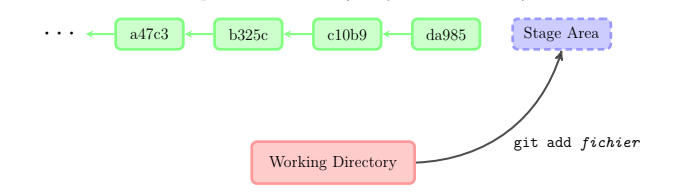
\includegraphics[width=\linewidth]{img/depot-git-add.png}
	\caption{État du dépôt lors de l'ajout d'un fichier à la zone de transit}
	\label{fig:git-add}
\end{figure}

\begin{Exercice}*{Renommer un fichier (version longue)}
	\begin{steps}
		
	\item La classe s'appelle \texttt{main}, ce qui n'est pas un bon choix de
		nom. Renommez la classe en \texttt{Main} (sans renommer le fichier pour
		l'instant). 
		\begin{itemize}
			\item Observez le résultat de \texttt{git status}.
			\item Faites un nouveau \texttt{git add main.java} et observez le
				résultat. 
		\end{itemize}

	\item Si la classe s'appelle \texttt{Main}, le fichier doit s'appeler
		\texttt{Main.java}. Pour le renommer, vous entrez naturellement la
		commande \texttt{mv main.java Main.java}. Faites le et observez le 
		résultat avec un \texttt{git status}.

		Git vous signale que le fichier \texttt{main.java} est supprimé et
		qu'un nouveau fichier \texttt{Main.java} — non suivi — existe. 

	\item Pour ajouter le nouveau fichier, vous entrez naturellement la commande 
		\texttt{git add Main.java}. Faites le et observez le résultat.  

		Git vous dit alors qu'un nouveau fichier \texttt{Main.java} existe, que
		le fichier \texttt{main.java} est modifié et que sa suppression n'est
		pas validée ! 
		
	\item Vous entrez alors la commande \texttt{git add main.java} pour valider
		la suppression. Faites le et observez le résultat. 

		Git vous montre (enfin) que le fichier a été renommé. Nous avions dit :
		« Version longue » n'est-ce-pas ? 

	\end{steps}
\end{Exercice}

\begin{Exercice}*{Renommer un fichier (version courte)}
	Finalement, cette classe pourrait s'appeler \texttt{Joxo} plutôt que 
	\texttt{Main}. 
	\begin{steps}
	
		\item Éditez le fichier et renommez la classe. 
		\item Renommez le fichier d'un simple 
			\texttt{git mv Main.java Joxo.java} et vérifiez le résultat avec un 
			\texttt{git status}… et un \texttt{ls}. 

	\end{steps}
\end{Exercice}



\section{Comparaison de \textit{commits} et de zones}

Nous avons déjà vu comment comparer des \textit{commits} entre eux. Voyons comment
comparer la zone de travail, la zone de transit et des \textit{commits}. La figure \vref{fig:git-diff} facilitera votre compréhension. 

\bigskip
\begin{colxbox}[colback=white,drop fuzzy shadow]
	\begin{verbatim}
	git diff
	    Compare la zone de transit avec la zone de travail
	git diff --staged
	    Compare le dernier commit avec la zone de transit
	git diff <id>
	    Compare le commit id avec la zone de travail
	git diff --staged <id>
	    Compare le commit id avec la zone de transit
	git diff <id1> <id2>
	    Compare le commit id1 avec le commit id2
	\end{verbatim}
\end{colxbox}
\bigskip

\begin{figure}[h]
	\centering
	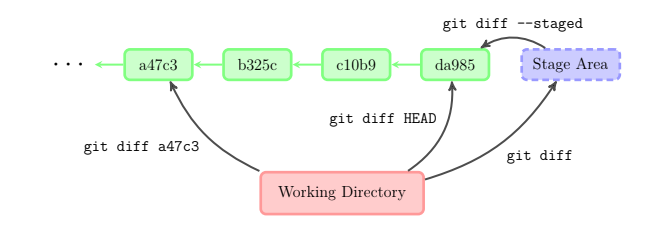
\includegraphics[width=\linewidth]{img/depot-git-diff.png}
	\caption{Différentes commandes de comparaisons}
	\label{fig:git-diff}
\end{figure}

\begin{Exercice}*{Comparaison zone de travail et zone de transit}
	\begin{steps}
		
	\item Éditez le fichier \texttt{Joxo.java} et ajoutez un commentaire javadoc
		pour la classe. 
	\item Comparez la zone de travail et la zone de transit avec \texttt{git diff}.
	
		Git vous montre l'ajout du commentaire javadoc.    

	\end{steps}
	
	
\end{Exercice}

\pagebreak
\begin{Exercice}*{Comparaison zone de travail et dernier commit}
	\begin{steps}
		
		\item Comparez la zone de travail et le dernier \textit{commit} avec l'une des
			deux méthodes suivantes : 
			\begin{itemize}
				\item \texttt{git diff HEAD} puisque le dernier \textit{commit} s'appelle 
					\texttt{HEAD};
				\item \texttt{git log -{}-oneline} pour trouver le numéro du dernier
					commit, suivi de \texttt{git diff bca37}.
			\end{itemize}

			Git vous montre l'ajout du commentaire javadoc ainsi que les 
			modifications apportées aux lignes trop longues. 

	\end{steps}
	
\end{Exercice}

\begin{Exercice}*{Comparaison zone de transit et dernier commit}
	\begin{steps}
		
		\item Comparez la zone de transit et le dernier \textit{commit} en ajoutant 
			\texttt{-{}-staged} aux dernières commandes. 

			Git ne vous montre plus l'ajout du commentaire javadoc qui est la
			modification dans la zone de travail mais uniquement les
			modifications apportées aux lignes trop longues du commit
			\texttt{bca37}. 

	\end{steps}
	
\end{Exercice}


\section{Création de \textit{commits}}

\begin{colxbox}[colback=white,drop fuzzy shadow]
	\begin{verbatim}
	git commit
	    Commite les changements en ouvrant l'éditeur par défaut. 

	    -m <message>
	        Commite directement les changements en utilisant le message 
	        passé en paramètre comme message de commit. 
	\end{verbatim}
\end{colxbox}
\bigskip 

Une fois les fichiers ajoutés à la zone de transit et les dernières
vérifications faites, nous pouvons enfin \textit{commiter} les fichiers pour
les placer dans le dépôt local. 

\begin{figure}[h]
	\centering
	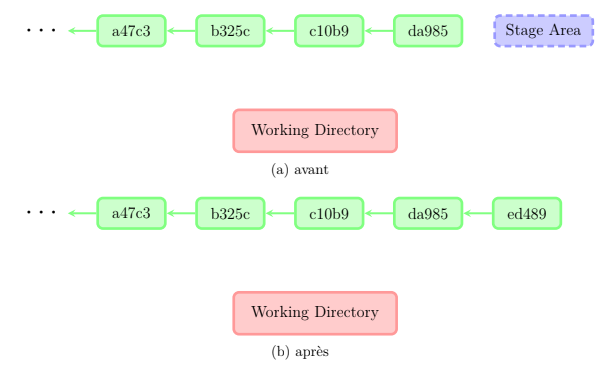
\includegraphics[width=\linewidth]{img/depot-git-commit.png}
	\caption{Situation d'un \textit{commit} « avant / après » }
	\label{fig:git-commit}
\end{figure}

L'opération terminée, git affiche un message contenant, entre autres, l'identifiant court du \textit{commit}, la première ligne de message et le nombre de changements. 

\pagebreak
Par exemple~:

\begin{verbatim}
[master ed489ba] First commit
1 file changed, 2 instertions(+)
\end{verbatim}

Si vous exécutez la commande \texttt{git commit} sans l’option \texttt{-m}, git
ouvre l’éditeur de texte par défaut du système\footnote{Sur de nombreux
	systèmes, cet éditeur de texte par défaut est \texttt{vim}. Son utilisation
	n’est pas intuitive. Si vous préférez nano, la commande \texttt{git config
	-{}-global core.editor nano} demandera à git d'enregistrer votre choix.
} pour permettre l’écriture du message. Il est ainsi possible d’écrire un
message avec une explication sur plusieurs lignes. 

Il n’y a pas de contrainte sur la forme des messages. Néanmoins, la convention
la plus utilisée est de commencer le message par une courte ligne de moins
d’une cinquantaine de caractères, suivie d’une ligne vide puis d’une
description complète. La première ligne servira de titre, par exemple, dans un
\texttt{git log -{}-oneline}. 



\begin{Exercice}*{Commit de nos changements}
	Notre dépôt contient un changement dans la zone de transit et un changement
	dans la zone de travail. Nous allons faire deux commits. 
	\begin{steps}
		
	\item Dans la zone de transit se trouve le changement concernant la
		longueur des lignes. Faites un \textit{commit} avec \texttt{git
			\textit{commit} -m "Correction de la longueur des lignes"}

		Vérifiez que le \textit{commit} est bien fait avec un \texttt{git log} par
		exemple. 

	\item Occupons nous du \textit{commit} concernant la javadoc dont les
		modifications se trouvent uniquement dans la zone de travail. Que
		faut-il faire ? 

		\begin{itemize}

			\item Ajoutez les changements dans la zone de transit avec
				\texttt{git add Joxo.java}

			\item Commitez avec un \texttt{git commit}.

				Git ouvre l'éditeur par défaut. Écrivez un message court suivi
				d'une message long présentant votre commit. 

		\end{itemize}

	\end{steps}
\end{Exercice}



\section{Publication des changements}

\bigskip
\begin{colxbox}[colback=white,drop fuzzy shadow]
	\begin{verbatim}
	git push 
	    Pousse à partir du dépôt local vers le dépôt distant. 
	git pull
	    Tire à partir du dépôt distant vers le dépôt local.
	\end{verbatim}
\end{colxbox}
\bigskip

Après les \textit{commits} de la section précédente, le dépôt devrait avoir cette allure : 

\begin{alltt}
\color{brown}commit 210eb38e9648bcabcd5bf9f59bfec1cffd714de1 (\color{blue}HEAD ->\color{green} master\color{brown})\color{black}
Author: Pierre Bettens (pbt) <pbettens@he2b.be>
Date:   Fri Nov 15 11:27:36 2019 +0100
 
     ajout de la javadoc
     
     Ajout d'une javadoc et d'un commentaire de \textit{commit} un peu plus long.
 
\color{brown}commit 77e542da5b02de89f6898a9f0ccafee9a7090821\color{black}
Author: Pierre Bettens (pbt) <pbettens@he2b.be>
Date:   Fri Nov 15 11:25:26 2019 +0100
 
     Correction de la longueur des lignes
 
\color{brown}commit bca37893fc1e29e6dd0a7b0bc292c6cf8aba624c (\color{red!80!black}origin/master, origin/HEAD\color{brown})\color{black}
Author: denis <denisname@users.noreply.github.com>
Date:   Thu Oct 17 15:25:30 2019 +0200
 
     Fixe test si le joueur gagne en oblique
     
     fixes #3
\end{alltt}

La première ligne, montre que le \textit{commit} \texttt{210eb} est le dernier commit :
\texttt{HEAD}. Le \textit{commit} \texttt{bca37} est étiqueté \textbf{origin/master} et
est le dernier \textit{commit} connu du dépôt distant.

Pour synchroniser le dépôt local avec le dépôt distant, il faut téléverser
(\textit{uploader}) le dépôt local (ses commits) vers le dépôt distant. 

\begin{Exercice}*{Mettre à jour le dépôt distant}
	\begin{steps}

	\item Faites un \texttt{git push} et vérifiez ensuite que les changements
		ont bien été répercutés sur le dépôt distant (à l'adresse que vous
		aviez notée). Voir figure \vref{fig:git-push}.
	
	\end{steps}
\end{Exercice}

\begin{figure}[h]
	\centering
	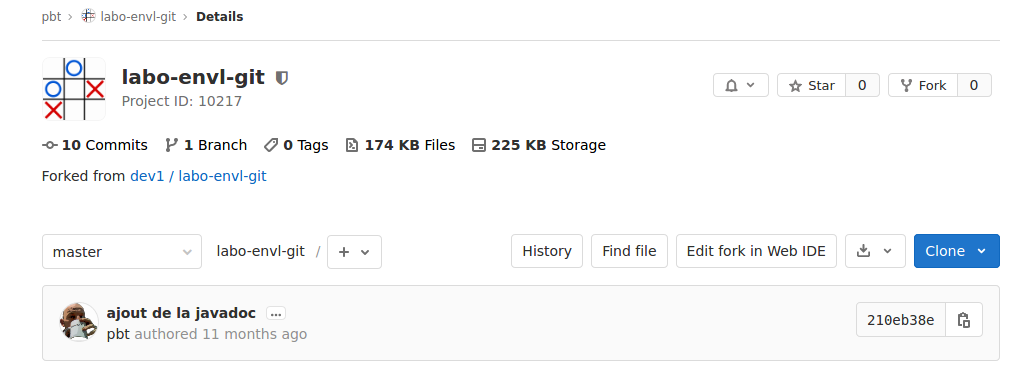
\includegraphics[width=\linewidth]{img/depot-distant-apres-1.png}
	Page du dépôt montrant le dernier commit.
	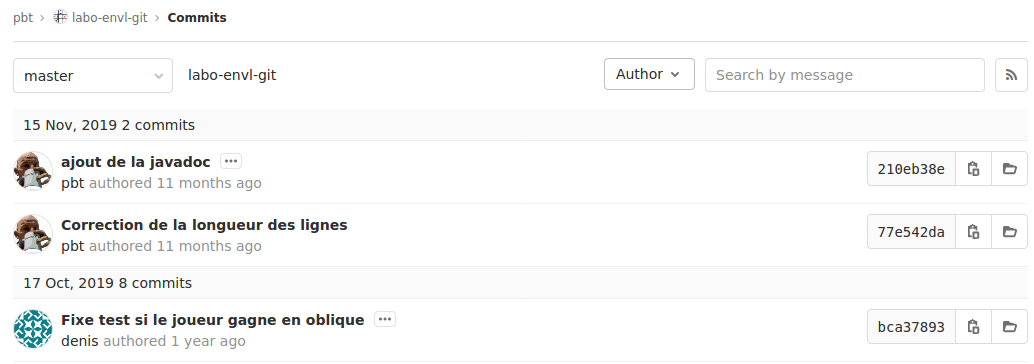
\includegraphics[width=\linewidth]{img/depot-distant-apres-2.png}
	Extrait de la liste des commits.
	\caption{Situation du dépôt distant après le \texttt{push}}
	\label{fig:git-push}
\end{figure}

\begin{alertit}{Rappel}
Lors d'un travail à plusieurs ou sur des machines différentes, il est
\textbf{indispensable} de s'assurer que le dépôt local est à jour avec le dépôt
distant en exécutant un \texttt{git pull} \textbf{avant} de commencer à travailler. 
\end{alertit}


\begin{faq}

	\textbf{J'ai du entrer mes identifiants lors du \texttt{clone} et lors du
	\texttt{push}. Faut-il faire ça à chaque fois ? }
	\medskip

	Oui et il faudra le faire aussi lors l'un \texttt{pull}. 

	Pour ne plus le faire, il est possible — et conseillé — de « déposer une
	clé ssh sur le serveur ». Voir sur le serveur gitlab de l'ESI
	\textit{Profile / Settings / SSH Keys}. Les informations sur comment faire se
	trouve en cliquant sur \href{https://git.esi-bru.be/help/ssh/README}
	{\textit{Generate it}}

	\bigskip
	\textbf{Je suis allé voir le répertoire \texttt{.git} comme conseillé. J'ai également 
	vu un fichier \texttt{.gitignore} qu'est-ce que c'est ?}
	\medskip

	Ce fichier contient des règles demandant à git d'ignorer certains fichiers du
	dépôt local. 


\end{faq}


\end{document}
